\documentclass{article}
\usepackage{graphicx}  % For including images
\usepackage{Sweave}    % For Sweave integration
\usepackage{amsmath}

\title{Integración en la UE: Resultados}
\author{Alba Nuez Vilà}
\date{Julio 2024}

\begin{document}
\Sconcordance{concordance:Informe_resultados.tex:Informe_resultados.Rnw:1 30 1 1 27 1 %
2 8 1}

\maketitle

\section{Actitud hacia los demás e inmigración}

\begin{center}
\emph{¿Cómo varía la actitud hacia los demás en diferentes países de la UE? ¿Cómo se correlaciona con la percepción del bienestar en relación con la inmigración?}
\end{center}

Las actitudes sociales y la percepción sobre la inmigración se influencian mutuamente. Entender cómo se dan estas relaciones puede ser crucial para mejorar la cohesión social y formular políticas de integración efectivas.

La variable ``actitud hacia los demás'' se obtiene calculando el promedio de las variables ``confianza'', ``honestidad'' y ``ayuda'', como puede observarse en la siguiente fórmula...

\[
\text{actitud hacia los demás} = \frac{\text{confianza} + \text{honestidad} + \text{ayuda}}{3}
\]

Estas variables están codificadas en una escala Likert, presentan patrones de respuesta similares y abordan cuestiones relacionadas (\textit{ver más detalle en el documento de planificación}). Esta variable varía de 0 a 10, donde 0 indica una actitud muy negativa hacia los demás y 10 una actitud muy positiva. 

A nivel europeo, la distribución de esta variable muestra que la mayoría de encuestados presentan una actitud positiva hacia los demás, con una clara tendencia a valores superiores a 5.

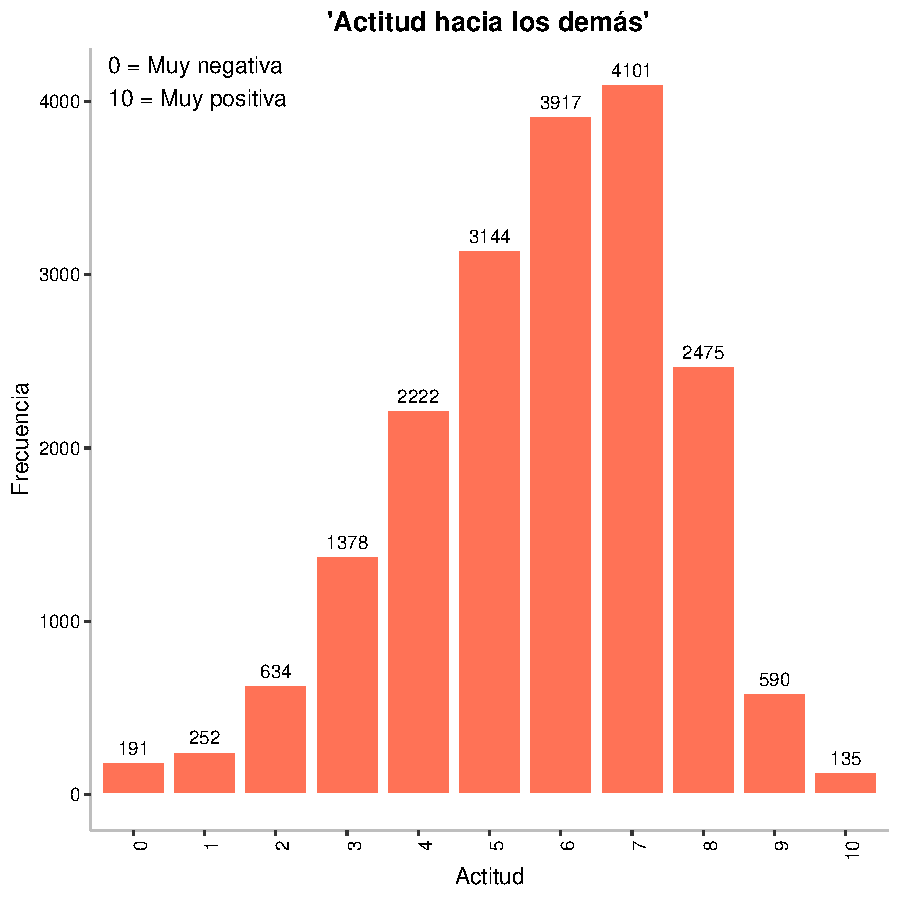
\includegraphics{Informe_resultados-histogram}

La actitud hacia los demás parece estar fuertemente influenciada por el país de origen del encuestado. Según el mapa de calor, los encuestados de Eslovaquia (SK) y Hungría (HU) tienden a mostrar una actitud menos favorable hacia los demás, con niveles de confianza, honestidad y ayuda por debajo de 5. En contraste, los encuestados austriacos (AT) muestran una actitud más positiva, con una respuesta predominante de 7 en estas variables.


\section{Adopción LGTBQ+}

% Add content for Part 2 here

\end{document}
